\documentclass{article} % For LaTeX2e
\usepackage{nips14submit_e,times}
\usepackage{hyperref}
\usepackage{url}
\usepackage{graphicx}
\usepackage{caption}
\usepackage{subcaption}
\usepackage{natbib}

\newenvironment{itemizedense}{
\begin{itemize}
  \setlength{\itemsep}{1pt}
  \setlength{\parskip}{0pt}
  \setlength{\parsep}{0pt}
}{\end{itemize}}

%\documentstyle[nips14submit_09,times,art10]{article} % For LaTeX 2.09

\title{DS-GA-1008 Assignment 2: Team LongCat}

\author{
Catherine Olsson, Long Sha, and Kevin Brown \\
}

\newcommand{\fix}{\marginpar{FIX}}
\newcommand{\new}{\marginpar{NEW}}

\nipsfinalcopy % Uncomment for camera-ready version

\begin{document}

\maketitle

\begin{abstract}
Current methods for image classification rely on large sets of labeled images.
However, there are massively many more unlabeled images readily available. To
evaluate the utility of unlabeled datasets to improve classiication performance
on labeld images, we implemented two main strategies: one basic
supervised-learning strategy, and one unsupervised-feature-learning strategy
based on Dosovitskiy et al \cite{dos}, which performed best at $54.4\%$ compared with $48\%$ for the standard supervised-only convolutional net.
\end{abstract}

\section{Supervised-only network}

We normalized each pixel globally, by subtracting the global mean for each
channel, and dividing by the standard deviation of the train data. We created a
convolutional neural net with two stages of convolutional
filter-nonlinear-pooling architecture and a nonlinear rectifier, followed by a
standard two-layer neural network. The input layer contained $96*96*3$ neurons,
one per pixel and RGB value. Layers One and Two used $128$ convolutional filter
banks of size $5 \times 5 \times 3$ pixels by RGB values, and $5 \times 5$
nodes, respectively. The standard two-layer net was a fully connected linear
layer with a ten linear output nodes, one for each image class, optimized with
stochastic gradient descent and a negative log-likelihood loss function. We
used a dropout probably $0.5$, momentum $0.998$, weight decay $0$, and a
learning rate of $10^{-3}$. This network performed at $48\%$ on the test set. 

\section{Unsupervised feature-learning network}
\subsection{Overview of approach}

The unsupervised feature-learning approach proceeds in two steps. The first step is to learn a feature representation from the unlabeled data. This is achieved by generating ``surrogate classes'', each consisting of a single image patch with various distortions applied, and then training a network to discriminate these surrogate classes. The second step is to train a simple linear classifier on the true labeled data, after first transforming the labeled images to the new feature representation.

\subsection{Step 1: Unsupervised feature learning}

\subsubsection{Surrogate data generation}

A surrogate dataset is generated by transforming patches of images drawn from the unlabeled image set. For each of the $n$ surrogate classes, a random image is chosen, a candidate $32\times32$ seed patch is selected, and $m$ exemplar patches are generated by applying random transformations to the original image.

First, candidate seed patches were screened for having enough variation in intensity, to avoid selecting uniform feature-less patches. We achieved this by filtering each candidate patch with a simple horizontal and vertical gradient filter (namely ${{1, 0, -1}}$ and ${{1},{0},{-1}}$). We set a minimum threshold for the overall sum of the absolute values of the pixel intensities in the two filtered images. Candidate patches which did not surpass this threshold were rejected. We found that a setting of $600$ produced interesting patches without taking too long to complete the search. 

Second, we generated $m$ transformed patches by randomly applying the following transformations:

\begin{itemizedense}
\item Rotation: up to 20 degrees, i.e. 0.35 radians.
\item Contrast: Raise the S and V components to a power between 0.25 and 3; multiply by 0.7 through 1.4; add -0.1 to 0.1.
\item Hue: add a value between -0.1 and 0.1
\item Translation: within 0.2 of the patch size
\end{itemizedense}

We did not implement the PCA-based contrast transformation described in Dostovitskiy et al, because it was more complicated to implement. We also removed the scaling transformation described in Dostovitskiy et al. simply because it was buggy and causing problems, and we did not have time to fix it before submission. We believe our results would have been more robust and our filters more scale-invariant if we had succeeded at implementing the scale transformation. We also added a left-right flip, which unfortunately was not quite correctly implemented in that we applied it before extracting the patch rather than after; implementing this correctly may have gained us even better performance. Example patches drawn from three surrogate classes can be seen in Figure~\ref{figpatch}.

We experimented with using surrogate datasets with up to a number of surrogate classes ranging from 20 to 2000, each with 100 exemplars. Consistent with the the original paper, we found that including more classes improved performance; we did not vary the number of exemplars because 100 was shown to be sufficient in the paper. However, the total number of classes we were able to use was ultimately restricted by memory limitations in our current implementation. We could have used more classes if we did not load all the classes onto the GPU at once. We used the practical upper limit of 2000 classes and 100 exemplars for our final analysis. 

\begin{figure}[h]
\centering
\begin{subfigure}{0.2\textwidth}
  \centering
  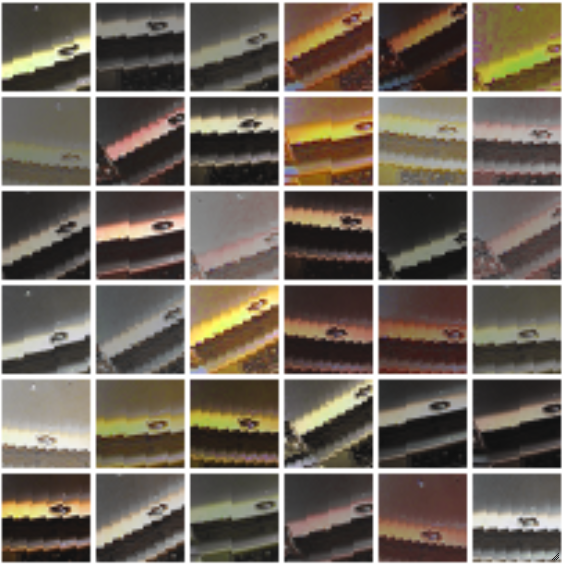
\includegraphics[width=\textwidth]{figs/patch_noflip_lines.png}
\end{subfigure}
\begin{subfigure}{0.2\textwidth}
  \centering
  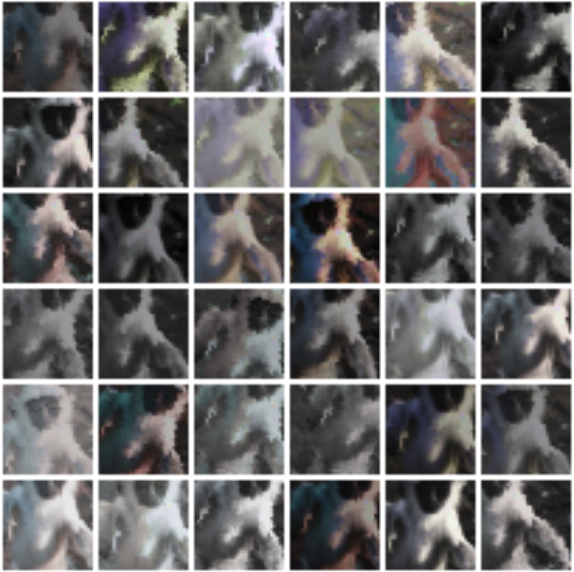
\includegraphics[width=\textwidth]{figs/patch_noflip_lemur.png}
\end{subfigure}
\begin{subfigure}{0.2\textwidth}
  \centering
  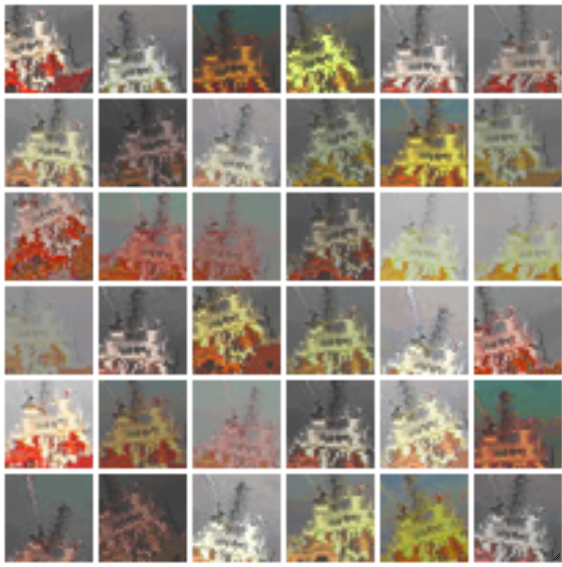
\includegraphics[width=\textwidth]{figs/patch_noflip_boattop.png}
\end{subfigure}
\caption{A selection of exemplars from three surrogate classes}
\label{figpatch}
\end{figure}

\subsubsection{Feature representation training}
The input of the feature representation training step is a surrogate dataset of $n$ generated classes, each with $m$ images ($32\times32$) derived from each class' seed patch.

For preprocessing, we computed the global mean and standard deviation of each channel based on the surrogate data. These statistics were used to zscore all the data. No additional normalization was performed.

The architecture of the surrogate-data classification model consists of three layers: (1) a 5x5 convolutional layer, stride of 1, with 128 filters, followed by a 2x2 max pooling layer; (2) a second 5x5 convolutional layer, stride of 1, with 256 filters, again followed by a 2x2 max pooling layer; (3) a fully connected layer, with 512 outputs, using dropout of 0.5; finally, a linear mapping to the 10 output classes.

We used stochastic gradient descent, with a learning rate of $1 \times 10^{-3}$, momentum of $0.998$, no weight decay, and a negative log likelihood loss function. We used a training set consisting of 75\% of the data, and a single validation set containing a random 25\% of the data, for all measurements and experiments except absolute last submission. We implemented the ability to perform ten-fold cross-validation, but did not use it for model selection because it proved to be very slow.

The learned first-layer filters from the unsupervised feature-learning step can be visualized in Figure~\ref{figfilt}.

\begin{figure}[h]
\centering
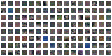
\includegraphics[width=0.5\textwidth]{figs/filter_sur.png}
\caption{The learned layer-1 filters}
\label{figfilt}
\end{figure}


\subsection{Step 2: Supervised classification}

\subsubsection{Feature representation transformation}

As in Dosovitskiy et al., the next step after learning a network that can produce a feature representation is to train a \emph{second} network to discriminate the true labeled classes based on the new feature embedding.

In Dosovitskiy et al., they ``applied the feature representation to images of arbitrary size by convolutionally computing the
responses of all the network layers except the top softmax. To each feature map, [they] applied the pooling method that is commonly used on the respective dataset: [...] 4-quadrant max-pooling, resulting in 4 values per feature map, which is the standard procedure on STL-10''. We interpreted this to mean that we should repeatedly run the learned model on $32\times32$ patches of each $96\times96$ image; concatenate the outputs of the first convolutional layer, the second convolutional layer, and the final fully connected layer, all together for a given patch; and pool the two spatial feature maps in four neighborhoods; to form an overall feature embedding of each patch.

We added some modifications to reduce the amount of computation. Overall, our process for applying the feature representation was the following:
\begin{itemizedense}
\item Perform spatial four-quadrant max pooling on the first layer and the second layer outputs (e.g. $128 \times 14 \times 14$ reduces to $128 \times 2 \times 2$ for the first layer).
\item Use a stride of 8 when extracting patches, which reduced the number of patches per image from $65\times65=4225$ patches to $9 \times 9 = 81$ patches.
\item Perform a second spatial four-quadrant max pooling to the overall representation, reducing it from $(9\times9) \times (128 \times 2 \times 2 + 256 \times 2 \times 2 + 512)$ features to $(2\times2) \times (128 \times 2 \times 2 + 256 \times 2 \times 2 + 512)$
\end{itemizedense}

Our final feature embedding per image was thus $8192$ dimensions.

\subsubsection{Supervised training}
The architecture we used at this stage was a simple linear layer (Dosovitskiy et al. used an SVM; we used \texttt{nn.Linear}). No additional preprocessing was performed. As before, we used negative log likelihood for our criterion.

\subsection{Results}

Overall, the highest performance we achieved was $54.4\%$ - however, this was on only 75\% of the data, because we did not get a chance to do a final pass with no validation set before the deadline. We will submit our final performance as soon as we are able.

To comment briefly on the effect of some choices we made: Adding the gradient cutoff in patch selection substantially improved our performance (from approximately 40\% to approximately 48\% on the validation set at the time we chose to include it). Also, we initially chose 128 filters per layer for all three layers in the unsupervised stage. When we increased the dimensionality of the layers to 128, 256, and 512, our performance improved (from approximately 48\% to approximately 53\% on the validation set).

\bibliographystyle{unsrt}
\bibliography{writeup}


\end{document}
